\documentclass[color=usenames,dvipsnames]{beamer}\usepackage[]{graphicx}\usepackage[]{color}
% maxwidth is the original width if it is less than linewidth
% otherwise use linewidth (to make sure the graphics do not exceed the margin)
\makeatletter
\def\maxwidth{ %
  \ifdim\Gin@nat@width>\linewidth
    \linewidth
  \else
    \Gin@nat@width
  \fi
}
\makeatother

\definecolor{fgcolor}{rgb}{0, 0, 0}
\newcommand{\hlnum}[1]{\textcolor[rgb]{0.69,0.494,0}{#1}}%
\newcommand{\hlstr}[1]{\textcolor[rgb]{0.749,0.012,0.012}{#1}}%
\newcommand{\hlcom}[1]{\textcolor[rgb]{0.514,0.506,0.514}{\textit{#1}}}%
\newcommand{\hlopt}[1]{\textcolor[rgb]{0,0,0}{#1}}%
\newcommand{\hlstd}[1]{\textcolor[rgb]{0,0,0}{#1}}%
\newcommand{\hlkwa}[1]{\textcolor[rgb]{0,0,0}{\textbf{#1}}}%
\newcommand{\hlkwb}[1]{\textcolor[rgb]{0,0.341,0.682}{#1}}%
\newcommand{\hlkwc}[1]{\textcolor[rgb]{0,0,0}{\textbf{#1}}}%
\newcommand{\hlkwd}[1]{\textcolor[rgb]{0.004,0.004,0.506}{#1}}%
\let\hlipl\hlkwb

\usepackage{framed}
\makeatletter
\newenvironment{kframe}{%
 \def\at@end@of@kframe{}%
 \ifinner\ifhmode%
  \def\at@end@of@kframe{\end{minipage}}%
  \begin{minipage}{\columnwidth}%
 \fi\fi%
 \def\FrameCommand##1{\hskip\@totalleftmargin \hskip-\fboxsep
 \colorbox{shadecolor}{##1}\hskip-\fboxsep
     % There is no \\@totalrightmargin, so:
     \hskip-\linewidth \hskip-\@totalleftmargin \hskip\columnwidth}%
 \MakeFramed {\advance\hsize-\width
   \@totalleftmargin\z@ \linewidth\hsize
   \@setminipage}}%
 {\par\unskip\endMakeFramed%
 \at@end@of@kframe}
\makeatother

\definecolor{shadecolor}{rgb}{.97, .97, .97}
\definecolor{messagecolor}{rgb}{0, 0, 0}
\definecolor{warningcolor}{rgb}{1, 0, 1}
\definecolor{errorcolor}{rgb}{1, 0, 0}
\newenvironment{knitrout}{}{} % an empty environment to be redefined in TeX

\usepackage{alltt}
%\documentclass[color=usenames,dvipsnames,handout]{beamer}


\usepackage[sans]{../../lab1}
\usepackage{bm}


\hypersetup{pdftex,pdfstartview=FitV}









%% New command for inline code that isn't to be evaluated
\definecolor{inlinecolor}{rgb}{0.878, 0.918, 0.933}
\newcommand{\inr}[1]{\colorbox{inlinecolor}{\texttt{#1}}}
\IfFileExists{upquote.sty}{\usepackage{upquote}}{}
\begin{document}


%\setlength\fboxsep{0pt}



\begin{frame}[plain]
  \huge
  \centering \par
  \textcolor{NavyBlue}{Introduction to Statistical Modeling} \\
  \vspace{1cm}
  \Large
%  November 2, 5, \& 7, 2018 \\
  FANR 6750 \\
  \vfill
  \large
  Richard Chandler and Bob Cooper
\end{frame}


\section{Motivation}



\begin{frame}
  \frametitle{Outline}
  \LARGE
   \only<1>{\tableofcontents[hideallsubsections]}
%   \only<2>{\tableofcontents[currentsection,hideallsubsections]}
\end{frame}




\begin{frame}
  \frametitle{Motivation}
  \large
  {\bf Why do we need this part of the course? \par}
  \pause
 \begin{columns}
   \begin{column}{0.75\paperwidth}
%\begin{enumerate}[<+- | visible@+->][\bf \color{PineGreen} (1)]
  \begin{itemize}%[<+->]
    \item[]
    \item<2-> We have been modeling all along
    \item[]
    \item<3-> Good experimental design + ANOVA is often the most direct
      route to causal inference
    \item[]
    \item<4-> However, it isn't always possible (or even desirable) to
      control some aspects of the system being investigated
    \item[]
    \item<5-> When manipulative experiments aren't 
      possible, observational studies
      and predictive models can be the next best option
  \end{itemize}
  \end{column}
  \begin{column}{0.19\paperwidth}
    \uncover<6->{
      
\includegraphics[width=\textwidth]{figs/Pearl_Causality} \\
      \vfill
      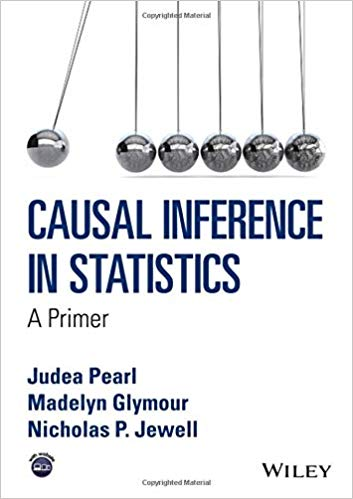
\includegraphics[width=\textwidth]{figs/Pearl_Primer} \\
    }
\end{column}
 \end{columns}
\end{frame}




\begin{frame}
  \frametitle{What is a model?}
    {\bf Definition} \\
    A model is an abstraction of reality used to describe the
    relationship between two or more variables \par
    \pause
    \vfill %\vspace{0.5cm}
    % \uncover<2->{
    {\bf Types of models}
    \begin{itemize}
      \item Conceptual
      \item Mathematical
      \item Statistical
    \end{itemize}
  \pause
  \vfill
  \begin{columns}%[t]
    \begin{column}[T]{0.75\textwidth}
      {\bf Cautionary note} \\
      ``All models are wrong but some are useful'' \\ (George Box, 1976) %\\
    \end{column}
    \begin{column}[T]{0.15\textwidth}
%      \uncover<3->{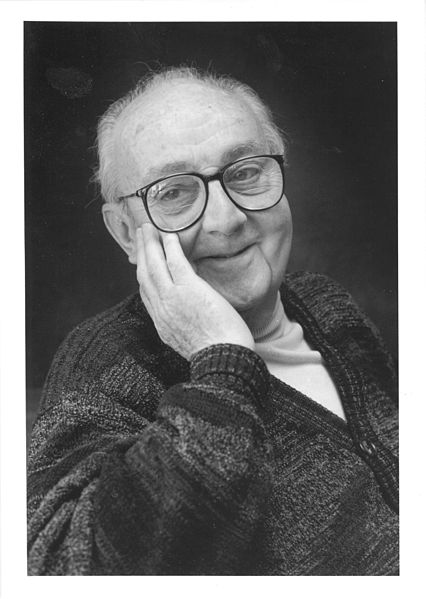
\includegraphics[width=\textwidth]{figs/Box}} \\
      {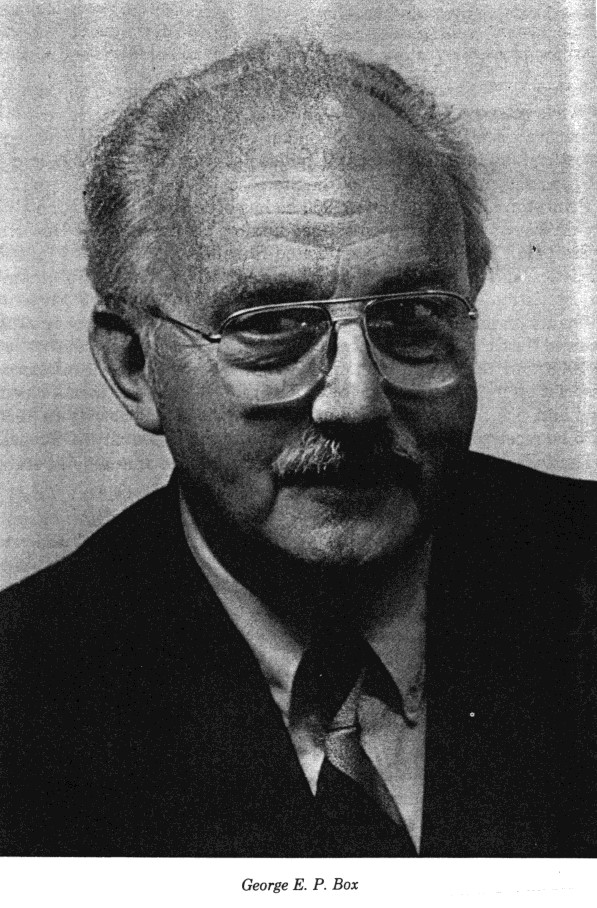
\includegraphics[width=\textwidth]{figs/Box2}} \\
    \end{column}
  \end{columns}
\end{frame}




\begin{frame}
  \frametitle{Statistical models}
  \large
  {\bf What are they \alert{useful} for?}
  \begin{itemize}%[<+->]
    \item[]
    \item<2-> Formalizing hypotheses using math and probability
    \item[]
    \item<3-> Evaulating hypotheses by confronting models with data
    \item[]
    \item<4-> Predicting unobserved (including future) outcomes
  \end{itemize}
  \vfill
  \centering
  \uncover<5->{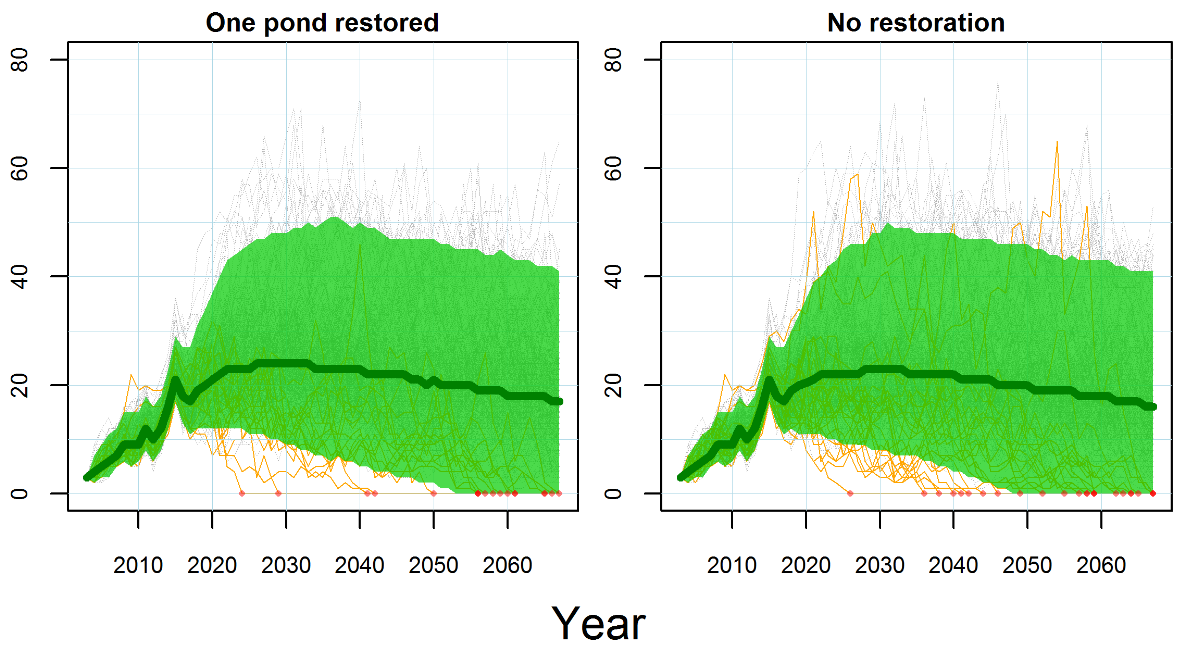
\includegraphics[width=0.6\textwidth]{figs/lich-forecasts}} \\
\end{frame}




\begin{frame}
  \frametitle{Statistical models}
  \large
  {Unlike many other types of models, statistical models are fitted to data \\}
  \pause
  \vspace{12pt} %\vfill
  {Two important components: \\}
  \vspace{6pt}
%  \large
%  \begin{enumerate}[<+- | visible@+->][\bf \color{PineGreen} (1)]
  \begin{enumerate}[\normalsize \bf \color{gb} (1)]
    \large
    \item<2-> Deterministic component%(s)
      \begin{itemize}
        % \large
        \normalsize
        \item Equation for the expected value of the response
          variable %, denoted $\mathbb{E}(y)$
      \end{itemize}
    \item[]
    \item<3-> Stochastic component %(s)
      \begin{itemize}
%        \large
        \normalsize
        \item<3-> Probability distribution %(s)
          describing the differences
          between the expected values and the observed values
        \item<4-> In parametric statistics, we assume we know the
          distribution, but not the parameters of the distribution
      \end{itemize}
  \end{enumerate}
\end{frame}




%% \begin{frame}
%%   \frametitle{Example}
%%   {\bf Motivation \\}
%%   Prey numbers appear to be declining in the core of the Florida panther's range \\
%%   \pause
%%   \vfill
%%   {\bf Questions \\}
%%   How do predation, changing hydrology and hunting regulations
%%   influence white-tailed deer population viability?
%% \end{frame}


%% \begin{frame}
%%   \frametitle{Example -- South Florida Deer Study}
%% %  \begin{center}
%% %  \vspace{-8mm}
%%   \begin{columns}
%%     \begin{column}{0.6\textwidth}
%% %      \large
%%         \normalsize
%%       {\bf Objectives}
%%       \begin{enumerate}
%%         \normalsize
%%         \item[{\bf (1)}] Understand how deer populations are influenced by:
%%         \begin{itemize}
%% %          \large
%%         \normalsize
%%           \item Predation
%%           \item Hydrology
%%           \item Hunting
%%         \end{itemize}
%%         \item[{\bf (2)}] Develop a camera-based monitoring program
%%       \end{enumerate}
%%     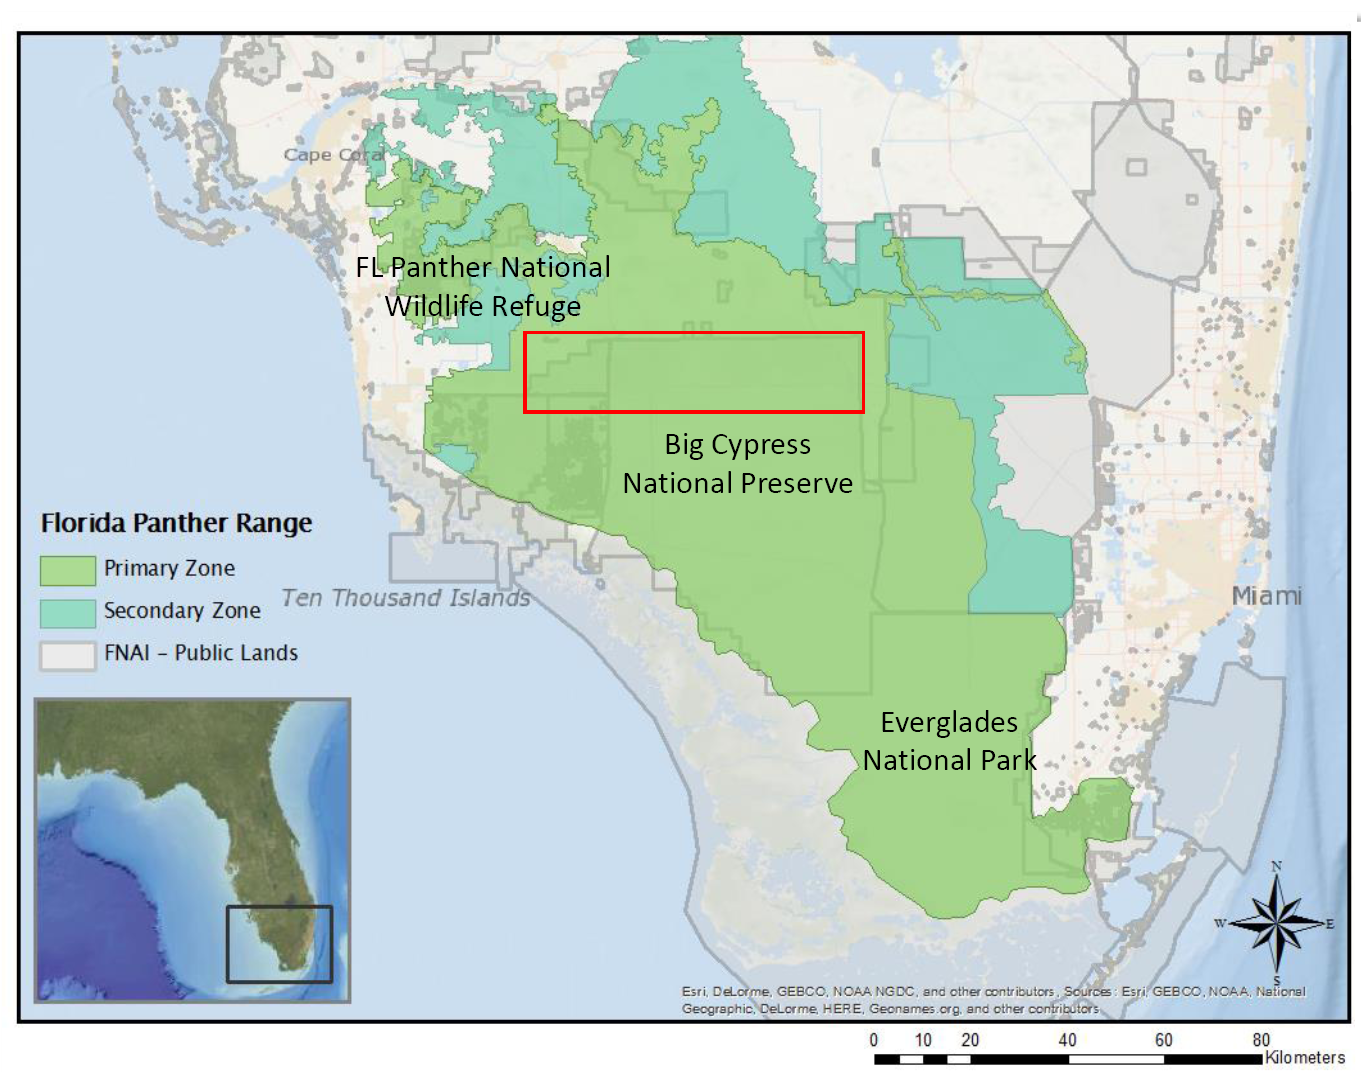
\includegraphics[width=0.9\textwidth]{figs/FL-study-area} \\ \vfill
%%     \end{column}
%%     \begin{column}{0.4\textwidth}
%%       \fbox{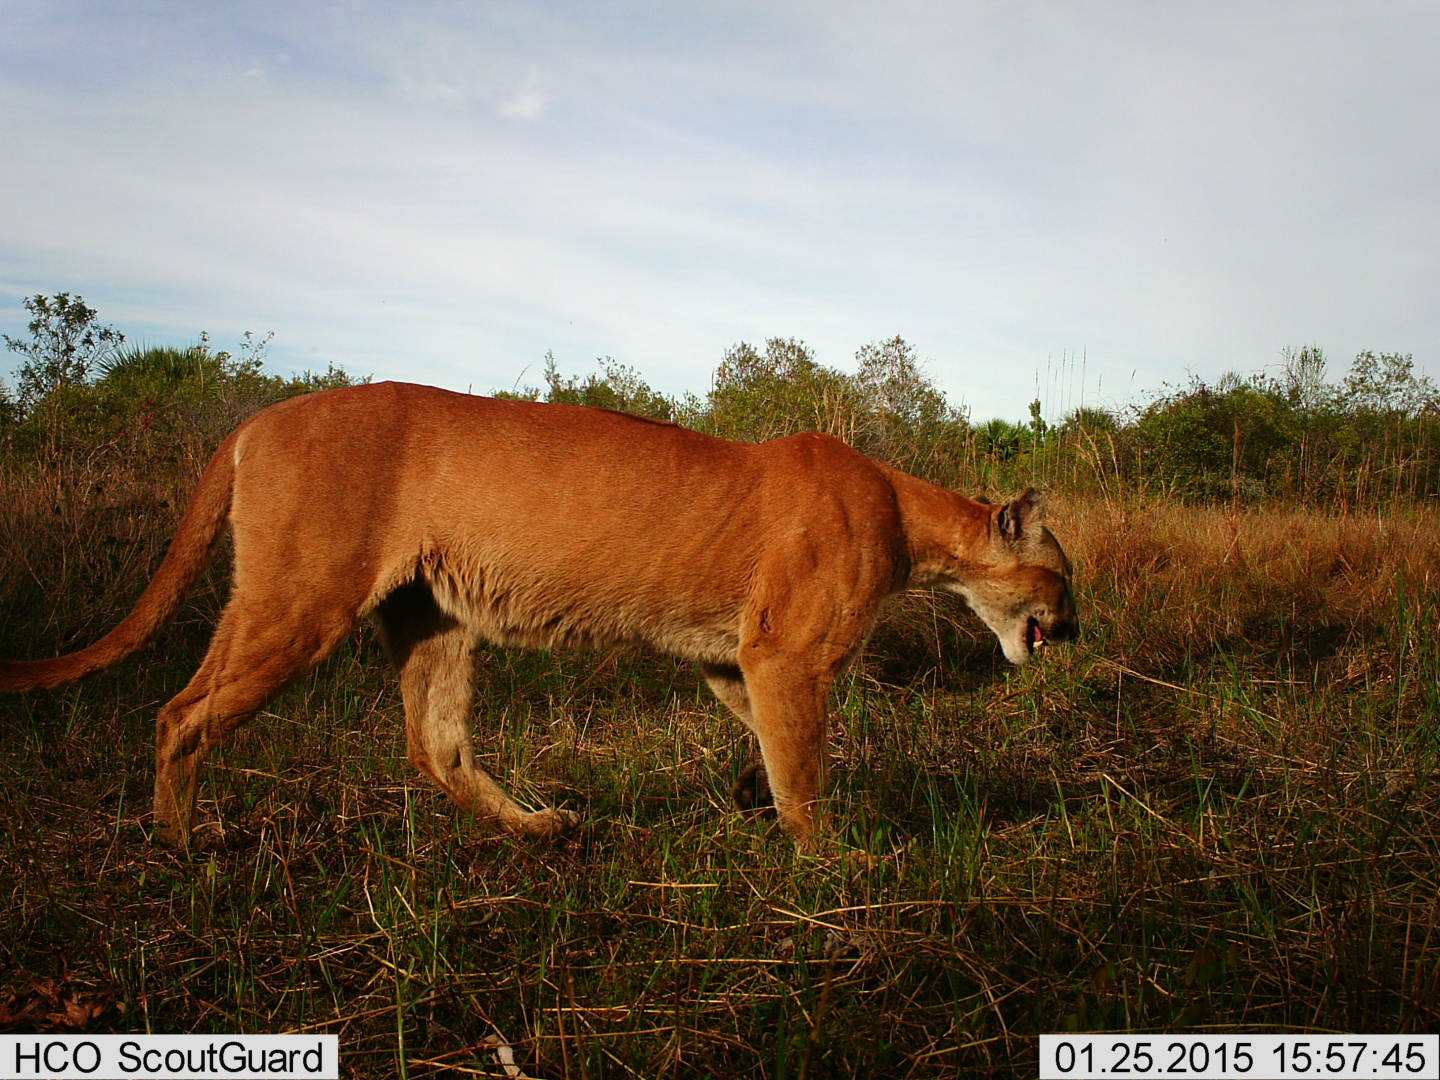
\includegraphics[width=\textwidth]{figs/puma1}} \\ \vfill
%%       \fbox{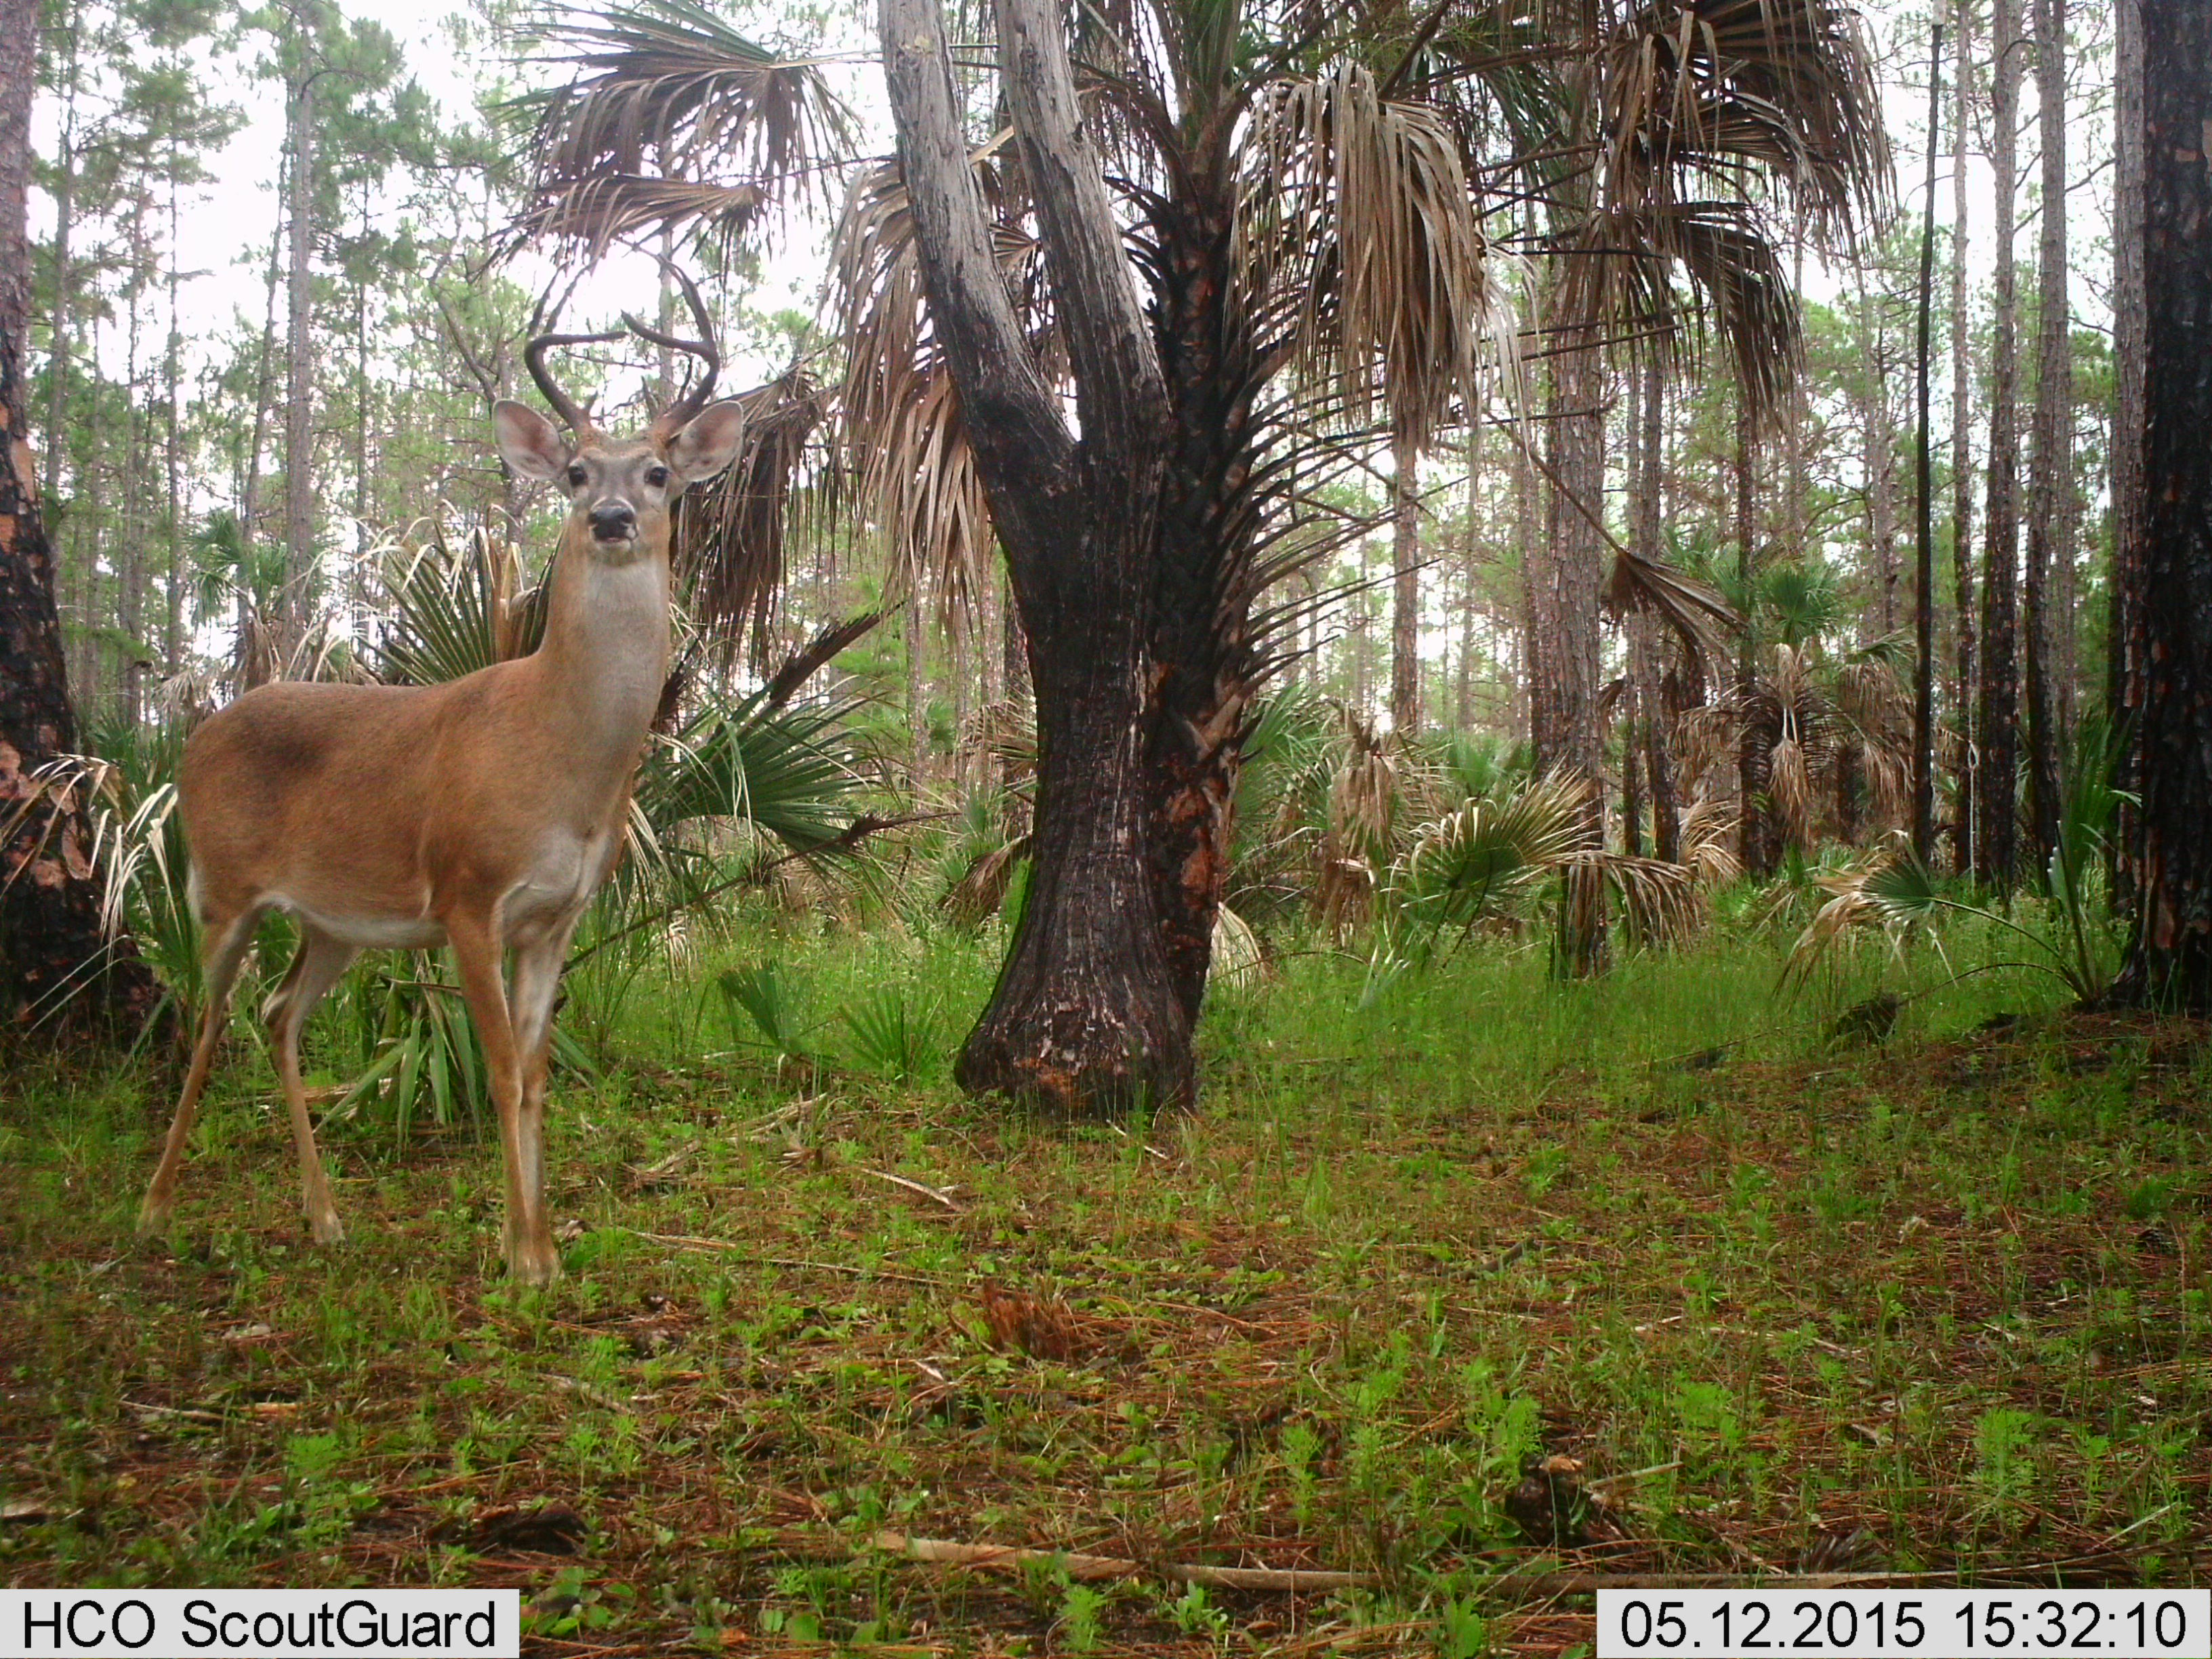
\includegraphics[width=\textwidth]{figs/2015-05-12-15-32-13_FP39}}
%%     \end{column}
%%   \end{columns}
%% %  \end{center}
%% \end{frame}









\section{Linear models}



\begin{frame}
  \frametitle{Outline}
  \LARGE
   \tableofcontents[currentsection,hideallsubsections]
\end{frame}



\begin{frame}[fragile]
  \frametitle{Is this a linear model?}
\[
y = 20 + 0.5 x
\]

\begin{center}
  \includegraphics[width=0.6\textwidth]{figure/linmod1-1}
\end{center}
\end{frame}




\begin{frame}[fragile]
  \frametitle{Is this a linear model?}
\[
y = 20 + 0.5 x - 0.3 x^2
\]

\begin{center}
  \includegraphics[width=0.6\textwidth]{figure/linmod2-1}
\end{center}
\end{frame}



\begin{frame}
  \frametitle{Linear models}
  All fixed-effects regression and ANOVA models are linear models \\
  \vfill
  You must understand linear models before you can apply more advanced models such as GLMs, GAMS, GLMMs, etc\dots
  \vfill
  \centering
  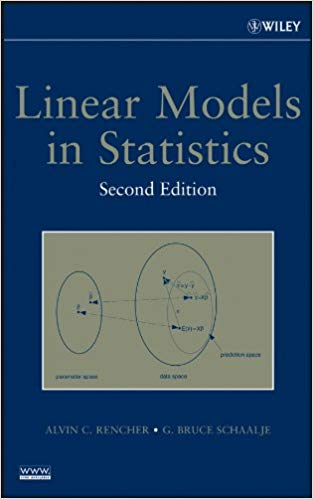
\includegraphics[width=0.25\textwidth]{figs/Rencher_Schaal_book} \hspace{1cm}
  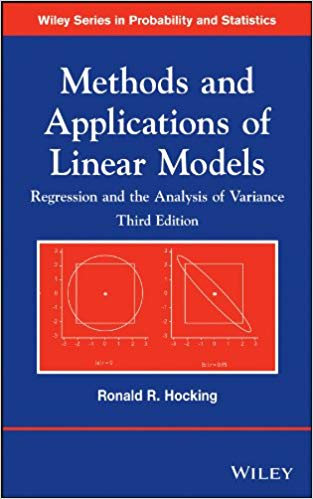
\includegraphics[width=0.25\textwidth]{figs/Hocking_book} \\
\end{frame}



\begin{frame}
  \frametitle{Linear model}
{\bf A linear model is an equation of the form:}

\[
y_i = \beta_0 + \beta_1 x_{i1} + \beta_2 x_{i2} + \ldots + \beta_p x_{ip} + \varepsilon_i
\]

where the $\beta$'s are coefficients, and the $x$ values are predictor
variables (or dummy variables for categorical predictors).
\pause

\vspace{0.5cm}

{\bf This equation is often expressed in matrix notation as:}

\[
{\bf y} = {\bf X} {\bm{\beta}} + {\bm \varepsilon}
\]

where $\bf X$ is a \alert{design matrix} and $\bm{\beta}$ is a
vector of coefficients. \pause More on matrix notation later\dots
\end{frame}


%\end{document}




\begin{frame}
  \frametitle{Interpretting the $\beta$'s}
You must be able to interpret the $\beta$
coefficients {\it for any model that you fit to your data}.
\pause
\vfill
A linear model might have dozens of continuous and categorical
predictors variables, with dozens of associated $\beta$ coefficients.
\pause
\vfill
%% Key points for interpretting $\beta$'s:
%% \begin{itemize}
%%   \item For continuous explano
%% \end{itemize}
Linear models can also include polynomial terms and interactions
\end{frame}


\begin{frame}[fragile]
  \frametitle{Interpretting the $\beta$'s}% for continuous explanatory variables}
  \small 
  The intercept $\beta_0$ is the expected value of $y$, when all $x$'s are 0 \\
  \pause
  \vfill
  If $x$ is a {\bf continuous} explanatory variable: %, $\beta$ is
  \begin{itemize}
    \item $\beta$ can usually be interpretted as a \textit{slope}
      parameter.
    \item In this case, $\beta$ is the
      change in $y$ resulting from a 1 unit change in $x$ (while
      holding the other predictors constant).
    \end{itemize}
\pause
\vfill

\centering
\begin{columns}
  \begin{column}{0.5\textwidth}
\begin{knitrout}\tiny
\definecolor{shadecolor}{rgb}{0.878, 0.918, 0.933}\color{fgcolor}\begin{kframe}
\begin{alltt}
\hlkwd{lm}\hlstd{(y}\hlopt{~}\hlstd{x)}
\end{alltt}
\begin{verbatim}
## 
## Call:
## lm(formula = y ~ x)
## 
## Coefficients:
## (Intercept)            x  
##       9.116        1.032
\end{verbatim}
\end{kframe}
\end{knitrout}
  \end{column}
  \begin{column}{0.4\textwidth}
  \includegraphics[width=\textwidth]{figure/linmod-1} \\
  \end{column}
\end{columns}
\end{frame}




\begin{frame}[fragile]
  \frametitle{\small Interpretting $\beta$'s for categorical explantory
    variables}
  Things are more complicated for {\bf categorical} explantory
  variables (i.e., factors) because they must be converted to dummy
  variables
  \pause
  \vfill
  There are many ways of creating dummy variables
  \pause
  \vfill
%  For a {\bf categorical} explanatory variable %, $\beta$ is
  In \R, the default method for creating dummy variables from
  unordered factors works like
  this: %unordered factors is called \inr{"contr.treatment"}
  \begin{itemize}
    \item One level of the factor is treated as a \alert{reference level}
    \item The reference level is associated with the intercept
    \item The $\beta$ coefficients for the other levels of the factor
      are differences from the reference level.
  \end{itemize}
  \pause
  \vfill
  The default method corresponds to:
\begin{knitrout}\small
\definecolor{shadecolor}{rgb}{0.878, 0.918, 0.933}\color{fgcolor}\begin{kframe}
\begin{alltt}
\hlkwd{options}\hlstd{(}\hlkwc{contrasts}\hlstd{=}\hlkwd{c}\hlstd{(}\hlstr{"contr.treatment"}\hlstd{,}\hlstr{"contr.poly"}\hlstd{))}
\end{alltt}
\end{kframe}
\end{knitrout}
\end{frame}




\begin{frame}[fragile]
  \frametitle{\small Interpretting $\beta$'s for categorical explantory
    variables}
  Another common method for creating dummy variables results in
  $\beta$'s that can be interpretted as the $\alpha$'s from the
  additive models that we saw earlier in the class.
  \pause
  \vfill
  With this method:
  \begin{itemize}
    \item The $\beta$ associated with each level of the factor is the
      difference from the intercept
    \item The intercept can be interpetted as the grand mean if the
      continuous variables have been centered
    \item One of the levels of the factor will not be displayed
      because it is redundant when the intercept is estimated
  \end{itemize}
  \pause
  \vfill
  This method corresponds to:
\begin{knitrout}\small
\definecolor{shadecolor}{rgb}{0.878, 0.918, 0.933}\color{fgcolor}\begin{kframe}
\begin{alltt}
\hlkwd{options}\hlstd{(}\hlkwc{contrasts}\hlstd{=}\hlkwd{c}\hlstd{(}\hlstr{"contr.sum"}\hlstd{,}\hlstr{"contr.poly"}\hlstd{))}
\end{alltt}
\end{kframe}
\end{knitrout}
\end{frame}



\section{Example}


\begin{frame}
  \frametitle{Outline}
  \LARGE
   \tableofcontents[currentsection,hideallsubsections]
\end{frame}



\begin{frame}[plain]
  \frametitle{Example}
  \Huge
  \begin{center}
    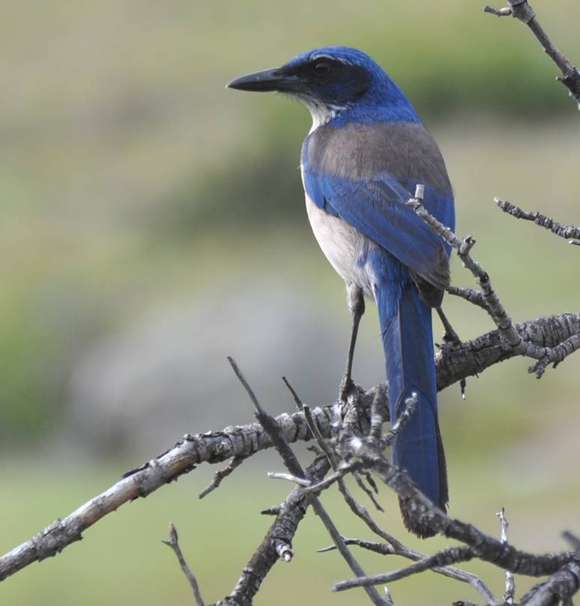
\includegraphics[width=0.5\textwidth]{figs/issj}
    The Island Scrub-Jay
  \end{center}
\end{frame}



\begin{frame}[plain]
  \frametitle{Example}
  \Huge
%  \begin{center}
  \centering
    Santa Cruz Island \\
  \begin{columns}
    \column{\dimexpr\paperwidth-20pt}
    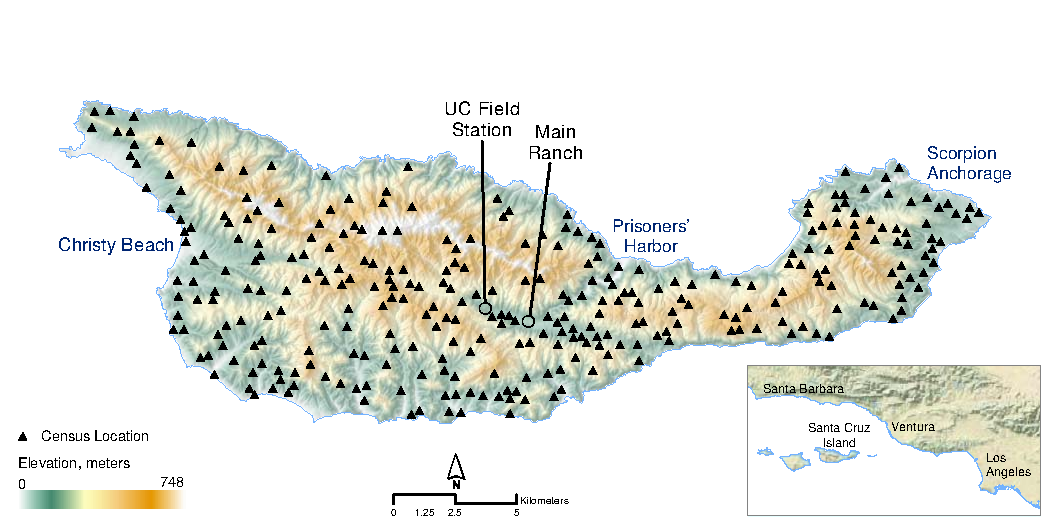
\includegraphics[width=\textwidth]{figs/Santa-Cruz} \\
  \end{columns}
%  \end{center}
\end{frame}




\begin{frame}[fragile]
  \frametitle{Santa Cruz Data}
  \footnotesize


{\bf Habitat data for all 2787 grid cells covering the island}
\begin{knitrout}
\definecolor{shadecolor}{rgb}{0.878, 0.918, 0.933}\color{fgcolor}\begin{kframe}
\begin{alltt}
\hlkwd{head}\hlstd{(cruz2)}
\end{alltt}
\begin{verbatim}
##          x       y elevation forest chaparral habitat seeds
## 1 230736.7 3774324       241      0         0     Oak   Low
## 2 231036.7 3774324       323      0         0    Pine   Med
## 3 231336.7 3774324       277      0         0    Pine  High
## 4 230436.7 3774024        13      0         0     Oak   Med
## 5 230736.7 3774024       590      0         0     Oak  High
## 6 231036.7 3774024       533      0         0     Oak   Low
\end{verbatim}
\end{kframe}
\end{knitrout}
\end{frame}



\begin{frame}[fragile]
  \frametitle{Maps of predictor variables}
%  {\bf Elevation}
  \scriptsize

\begin{columns}
  \column{\dimexpr\paperwidth-10pt}
  \includegraphics[width=\textwidth]{figure/elev-1}
\end{columns}
\end{frame}




\begin{frame}[fragile]
  \frametitle{Maps of predictor variables}
%  {\bf Forest cover}
  \scriptsize

\begin{columns}
  \column{\dimexpr\paperwidth-10pt}
  \includegraphics[width=\textwidth]{figure/forest-1}
\end{columns}
\end{frame}






\begin{frame}
  \frametitle{Questions}
  \large
%  \begin{enumerate}[<+- | visible@+->][\bf \color{PineGreen} (1)]
  \begin{enumerate}[\bf \color{PineGreen} (1)]
    \item How many jays are on the island?
    \item[]
    \item What environmental variables influence abundance?
    \item[]
    \item Can we predict consequences of environmental change?
  \end{enumerate}
\end{frame}



\begin{frame}[fragile]
  \frametitle{Maps of predictor variables}
%  {\bf Chaparral cover}

\begin{columns}
  \column{\dimexpr\paperwidth-10pt}
  \includegraphics[width=\textwidth]{figure/plots-1}
\end{columns}
\end{frame}




\begin{frame}[fragile]
  \frametitle{The (fake) jay data}
\begin{knitrout}\scriptsize
\definecolor{shadecolor}{rgb}{0.878, 0.918, 0.933}\color{fgcolor}\begin{kframe}
\begin{alltt}
\hlkwd{head}\hlstd{(jayData)}
\end{alltt}
\begin{verbatim}
##             x       y elevation forest chaparral habitat seeds jays
## 1895 240336.7 3765324       812   0.00      0.12     Oak   Med   37
## 1003 234636.7 3768024       182   0.00      0.29    Pine   Med   34
## 969  249336.7 3768324       791   0.15      0.16    Pine  High   38
## 1408 249336.7 3766824      1353   0.00      0.09    Pine   Med   42
## 2002 242136.7 3765024       746   0.01      0.54    Pine   Low   38
## 367  243336.7 3770724       988   0.08      0.17    Pine  High   40
\end{verbatim}
\end{kframe}
\end{knitrout}
\end{frame}




\begin{frame}[fragile]
  \frametitle{Simple linear regression}
\begin{knitrout}\scriptsize
\definecolor{shadecolor}{rgb}{0.878, 0.918, 0.933}\color{fgcolor}\begin{kframe}
\begin{alltt}
\hlstd{fm1} \hlkwb{<-} \hlkwd{lm}\hlstd{(jays} \hlopt{~} \hlstd{elevation,} \hlkwc{data}\hlstd{=jayData)}
\hlkwd{summary}\hlstd{(fm1)}
\end{alltt}
\begin{verbatim}
## 
## Call:
## lm(formula = jays ~ elevation, data = jayData)
## 
## Residuals:
##     Min      1Q  Median      3Q     Max 
## -4.2433 -1.4388  0.2374  1.5347  4.9672 
## 
## Coefficients:
##              Estimate Std. Error t value Pr(>|t|)    
## (Intercept) 33.318197   0.456375   73.01   <2e-16 ***
## elevation    0.008148   0.000508   16.04   <2e-16 ***
## ---
## Signif. codes:  0 '***' 0.001 '**' 0.01 '*' 0.05 '.' 0.1 ' ' 1
## 
## Residual standard error: 2.133 on 98 degrees of freedom
## Multiple R-squared:  0.7242,	Adjusted R-squared:  0.7214 
## F-statistic: 257.3 on 1 and 98 DF,  p-value: < 2.2e-16
\end{verbatim}
\end{kframe}
\end{knitrout}
\end{frame}


\begin{frame}[fragile]
  \frametitle{Simple linear regression}
\begin{knitrout}
\definecolor{shadecolor}{rgb}{0.878, 0.918, 0.933}\color{fgcolor}
\includegraphics[width=\maxwidth]{figure/pred1-1} 

\end{knitrout}
\end{frame}



\begin{frame}[fragile]
  \frametitle{Multiple linear regression}
\begin{knitrout}\scriptsize
\definecolor{shadecolor}{rgb}{0.878, 0.918, 0.933}\color{fgcolor}\begin{kframe}
\begin{alltt}
\hlstd{fm2} \hlkwb{<-} \hlkwd{lm}\hlstd{(jays} \hlopt{~} \hlstd{elevation}\hlopt{+}\hlstd{forest,} \hlkwc{data}\hlstd{=jayData)}
\hlkwd{summary}\hlstd{(fm2)}
\end{alltt}
\begin{verbatim}
## 
## Call:
## lm(formula = jays ~ elevation + forest, data = jayData)
## 
## Residuals:
##     Min      1Q  Median      3Q     Max 
## -4.3053 -1.4577  0.1757  1.5512  4.8988 
## 
## Coefficients:
##               Estimate Std. Error t value Pr(>|t|)    
## (Intercept) 33.3707514  0.4622909  72.186   <2e-16 ***
## elevation    0.0081741  0.0005101  16.025   <2e-16 ***
## forest      -1.8556417  2.3911829  -0.776     0.44    
## ---
## Signif. codes:  0 '***' 0.001 '**' 0.01 '*' 0.05 '.' 0.1 ' ' 1
## 
## Residual standard error: 2.137 on 97 degrees of freedom
## Multiple R-squared:  0.7259,	Adjusted R-squared:  0.7202 
## F-statistic: 128.4 on 2 and 97 DF,  p-value: < 2.2e-16
\end{verbatim}
\end{kframe}
\end{knitrout}
\end{frame}




\begin{frame}[fragile]
  \frametitle{Multiple linear regression}
\begin{knitrout}
\definecolor{shadecolor}{rgb}{0.878, 0.918, 0.933}\color{fgcolor}
\includegraphics[width=\maxwidth]{figure/pred2-1} 

\end{knitrout}
\end{frame}





\begin{frame}[fragile]
  \frametitle{One-way ANOVA}
\begin{knitrout}\scriptsize
\definecolor{shadecolor}{rgb}{0.878, 0.918, 0.933}\color{fgcolor}\begin{kframe}
\begin{alltt}
\hlstd{fm3} \hlkwb{<-} \hlkwd{lm}\hlstd{(jays} \hlopt{~} \hlstd{habitat,} \hlkwc{data}\hlstd{=jayData)}
\hlkwd{summary}\hlstd{(fm3)}
\end{alltt}
\begin{verbatim}
## 
## Call:
## lm(formula = jays ~ habitat, data = jayData)
## 
## Residuals:
##     Min      1Q  Median      3Q     Max 
## -8.9062 -3.1129 -0.1129  2.8871  8.8871 
## 
## Coefficients:
##             Estimate Std. Error t value Pr(>|t|)    
## (Intercept)   35.833      1.614  22.204   <2e-16 ***
## habitatOak     4.280      1.690   2.532   0.0129 *  
## habitatPine    4.073      1.759   2.316   0.0227 *  
## ---
## Signif. codes:  0 '***' 0.001 '**' 0.01 '*' 0.05 '.' 0.1 ' ' 1
## 
## Residual standard error: 3.953 on 97 degrees of freedom
## Multiple R-squared:  0.06237,	Adjusted R-squared:  0.04304 
## F-statistic: 3.226 on 2 and 97 DF,  p-value: 0.04401
\end{verbatim}
\end{kframe}
\end{knitrout}
\end{frame}




\begin{frame}[fragile]
  \frametitle{One-way ANOVA}

\centering
\includegraphics[width=0.8\textwidth]{figure/pred3-1} \\
\end{frame}





\begin{frame}[fragile]
  \frametitle{ANCOVA}
\begin{knitrout}\scriptsize
\definecolor{shadecolor}{rgb}{0.878, 0.918, 0.933}\color{fgcolor}\begin{kframe}
\begin{alltt}
\hlstd{fm4} \hlkwb{<-} \hlkwd{lm}\hlstd{(jays} \hlopt{~} \hlstd{elevation}\hlopt{+}\hlstd{habitat,} \hlkwc{data}\hlstd{=jayData)}
\hlkwd{summary}\hlstd{(fm4)}
\end{alltt}
\begin{verbatim}
## 
## Call:
## lm(formula = jays ~ elevation + habitat, data = jayData)
## 
## Residuals:
##     Min      1Q  Median      3Q     Max 
## -4.6171 -1.5698  0.0892  1.6378  4.3895 
## 
## Coefficients:
##              Estimate Std. Error t value Pr(>|t|)    
## (Intercept) 3.136e+01  8.622e-01  36.374  < 2e-16 ***
## elevation   8.179e-03  4.888e-04  16.731  < 2e-16 ***
## habitatOak  2.493e+00  8.651e-01   2.882  0.00488 ** 
## habitatPine 1.205e+00  9.096e-01   1.325  0.18827    
## ---
## Signif. codes:  0 '***' 0.001 '**' 0.01 '*' 0.05 '.' 0.1 ' ' 1
## 
## Residual standard error: 2.008 on 96 degrees of freedom
## Multiple R-squared:  0.7606,	Adjusted R-squared:  0.7531 
## F-statistic: 101.6 on 3 and 96 DF,  p-value: < 2.2e-16
\end{verbatim}
\end{kframe}
\end{knitrout}
\end{frame}



\begin{frame}[fragile]
  \frametitle{ANCOVA}
\begin{knitrout}
\definecolor{shadecolor}{rgb}{0.878, 0.918, 0.933}\color{fgcolor}
\includegraphics[width=\maxwidth]{figure/pred4-1} 

\end{knitrout}
\end{frame}





\begin{frame}[fragile]
  \frametitle{Continuous-categorical interaction}
\begin{knitrout}\tiny
\definecolor{shadecolor}{rgb}{0.878, 0.918, 0.933}\color{fgcolor}\begin{kframe}
\begin{alltt}
\hlstd{fm5} \hlkwb{<-} \hlkwd{lm}\hlstd{(jays} \hlopt{~} \hlstd{elevation}\hlopt{*}\hlstd{habitat,} \hlkwc{data}\hlstd{=jayData)}
\hlkwd{summary}\hlstd{(fm5)}
\end{alltt}
\begin{verbatim}
## 
## Call:
## lm(formula = jays ~ elevation * habitat, data = jayData)
## 
## Residuals:
##     Min      1Q  Median      3Q     Max 
## -4.5238 -1.5586  0.1117  1.6228  4.6687 
## 
## Coefficients:
##                        Estimate Std. Error t value Pr(>|t|)    
## (Intercept)           30.508235   1.592372  19.159  < 2e-16 ***
## elevation              0.009741   0.002495   3.904 0.000178 ***
## habitatOak             3.735717   1.689354   2.211 0.029437 *  
## habitatPine            1.568104   1.771844   0.885 0.378408    
## elevation:habitatOak  -0.002070   0.002580  -0.802 0.424382    
## elevation:habitatPine -0.001015   0.002611  -0.389 0.698402    
## ---
## Signif. codes:  0 '***' 0.001 '**' 0.01 '*' 0.05 '.' 0.1 ' ' 1
## 
## Residual standard error: 2.013 on 94 degrees of freedom
## Multiple R-squared:  0.7643,	Adjusted R-squared:  0.7518 
## F-statistic: 60.96 on 5 and 94 DF,  p-value: < 2.2e-16
\end{verbatim}
\end{kframe}
\end{knitrout}
\end{frame}




\begin{frame}[fragile]
  \frametitle{Continuous-categorical interaction}
\begin{knitrout}
\definecolor{shadecolor}{rgb}{0.878, 0.918, 0.933}\color{fgcolor}
\includegraphics[width=\maxwidth]{figure/pred5-1} 

\end{knitrout}
\end{frame}






\begin{frame}[fragile]
  \frametitle{Quadratic effect of elevation}
\begin{knitrout}\scriptsize
\definecolor{shadecolor}{rgb}{0.878, 0.918, 0.933}\color{fgcolor}\begin{kframe}
\begin{alltt}
\hlstd{fm6} \hlkwb{<-} \hlkwd{lm}\hlstd{(jays} \hlopt{~} \hlstd{elevation}\hlopt{+}\hlkwd{I}\hlstd{(elevation}\hlopt{^}\hlnum{2}\hlstd{),} \hlkwc{data}\hlstd{=jayData)}
\hlkwd{summary}\hlstd{(fm6)}
\end{alltt}
\begin{verbatim}
## 
## Call:
## lm(formula = jays ~ elevation + I(elevation^2), data = jayData)
## 
## Residuals:
##     Min      1Q  Median      3Q     Max 
## -4.2656 -1.4829  0.2837  1.5030  4.9863 
## 
## Coefficients:
##                  Estimate Std. Error t value Pr(>|t|)    
## (Intercept)     3.312e+01  7.311e-01  45.304  < 2e-16 ***
## elevation       8.774e-03  1.897e-03   4.624 1.16e-05 ***
## I(elevation^2) -3.742e-07  1.093e-06  -0.342    0.733    
## ---
## Signif. codes:  0 '***' 0.001 '**' 0.01 '*' 0.05 '.' 0.1 ' ' 1
## 
## Residual standard error: 2.143 on 97 degrees of freedom
## Multiple R-squared:  0.7245,	Adjusted R-squared:  0.7188 
## F-statistic: 127.6 on 2 and 97 DF,  p-value: < 2.2e-16
\end{verbatim}
\end{kframe}
\end{knitrout}
\end{frame}




\begin{frame}[fragile]
  \frametitle{Quadratic effect of elevation}
\begin{knitrout}
\definecolor{shadecolor}{rgb}{0.878, 0.918, 0.933}\color{fgcolor}
\includegraphics[width=\maxwidth]{figure/pred6-1} 

\end{knitrout}
\end{frame}






\begin{frame}[fragile]
  \frametitle{Interaction and quadratic effects}
  \vspace{-2mm}
\begin{knitrout}\tiny
\definecolor{shadecolor}{rgb}{0.878, 0.918, 0.933}\color{fgcolor}\begin{kframe}
\begin{alltt}
\hlstd{fm7} \hlkwb{<-} \hlkwd{lm}\hlstd{(jays} \hlopt{~} \hlstd{habitat} \hlopt{*} \hlstd{forest} \hlopt{+} \hlstd{elevation} \hlopt{+}
          \hlkwd{I}\hlstd{(elevation}\hlopt{^}\hlnum{2}\hlstd{),} \hlkwc{data}\hlstd{=jayData)}
\hlkwd{summary}\hlstd{(fm7)}
\end{alltt}
\begin{verbatim}
## 
## Call:
## lm(formula = jays ~ habitat * forest + elevation + I(elevation^2), 
##     data = jayData)
## 
## Residuals:
##     Min      1Q  Median      3Q     Max 
## -4.4245 -1.4311  0.0855  1.6472  4.4907 
## 
## Coefficients:
##                      Estimate Std. Error t value Pr(>|t|)    
## (Intercept)         3.022e+01  1.289e+00  23.444  < 2e-16 ***
## habitatOak          3.756e+00  1.225e+00   3.065  0.00286 ** 
## habitatPine         2.777e+00  1.266e+00   2.193  0.03086 *  
## forest              7.414e+01  4.636e+01   1.599  0.11322    
## elevation           7.519e-03  1.806e-03   4.162 7.08e-05 ***
## I(elevation^2)      3.438e-07  1.044e-06   0.329  0.74276    
## habitatOak:forest  -6.934e+01  4.660e+01  -1.488  0.14012    
## habitatPine:forest -7.693e+01  4.645e+01  -1.656  0.10107    
## ---
## Signif. codes:  0 '***' 0.001 '**' 0.01 '*' 0.05 '.' 0.1 ' ' 1
## 
## Residual standard error: 2.001 on 92 degrees of freedom
## Multiple R-squared:  0.7721,	Adjusted R-squared:  0.7547 
## F-statistic: 44.52 on 7 and 92 DF,  p-value: < 2.2e-16
\end{verbatim}
\end{kframe}
\end{knitrout}
\end{frame}



\begin{frame}[fragile]
  \frametitle{Predict jay abundance at each grid cell}
\begin{knitrout}
\definecolor{shadecolor}{rgb}{0.878, 0.918, 0.933}\color{fgcolor}\begin{kframe}
\begin{alltt}
\hlstd{E7} \hlkwb{<-} \hlkwd{predict}\hlstd{(fm7,} \hlkwc{type}\hlstd{=}\hlstr{"response"}\hlstd{,} \hlkwc{newdata}\hlstd{=cruz2,}
              \hlkwc{interval}\hlstd{=}\hlstr{"confidence"}\hlstd{)}
\end{alltt}
\end{kframe}
\end{knitrout}
\pause
\begin{knitrout}
\definecolor{shadecolor}{rgb}{0.878, 0.918, 0.933}\color{fgcolor}\begin{kframe}
\begin{alltt}
\hlstd{E7} \hlkwb{<-} \hlkwd{cbind}\hlstd{(cruz2[,}\hlkwd{c}\hlstd{(}\hlstr{"x"}\hlstd{,}\hlstr{"y"}\hlstd{)], E7)}
\hlkwd{head}\hlstd{(E7)}
\end{alltt}
\begin{verbatim}
##          x       y      fit      lwr      upr
## 1 230736.7 3774324 35.81133 34.95667 36.66599
## 2 231036.7 3774324 35.46495 34.49121 36.43868
## 3 231336.7 3774324 35.10958 34.09035 36.12882
## 4 230436.7 3774024 34.07706 32.67001 35.48412
## 5 230736.7 3774024 38.53521 37.91238 39.15803
## 6 231036.7 3774024 38.08461 37.46267 38.70655
\end{verbatim}
\end{kframe}
\end{knitrout}
\end{frame}


\begin{frame}[fragile]
  \frametitle{Map the predictions}
  \scriptsize

\begin{columns}
  \column{\dimexpr\paperwidth-10pt}
  \includegraphics[width=\textwidth]{figure/Ejay-1}
\end{columns}
\end{frame}




\begin{frame}[fragile]
  \frametitle{Map the predictions}
  \scriptsize

\begin{columns}
  \column{\dimexpr\paperwidth-10pt}
  \includegraphics[width=\textwidth]{figure/Ljay-1}
\end{columns}
\end{frame}




\begin{frame}[fragile]
  \frametitle{Map the predictions}
  \scriptsize

\begin{columns}
  \column{\dimexpr\paperwidth-10pt}
  \includegraphics[width=\textwidth]{figure/Ujay-1}
\end{columns}
\end{frame}




%% \begin{frame}[fragile]
%%   \frametitle{Future scenarios}
%%   {\bf What if the pine and oak disappear? \par}
%%   \pause
%%   \vspace{0.3cm}
%%   {\bf \dots assuming {\tt fm5} is the {\it correct} model}
%%   \pause
%%   \vspace{0.3cm}
%%   \footnotesize
%% <<>>=
%% future1 <- cruz2
%% future1$habitat[] <- "Bare"
%% future.pred1 <- predict(fm5, type="response", newdata=future1,
%%                         interval="confidence")
%% future.pred1 <- cbind(cruz2[,c("x","y")], future.pred1)
%% @
%% \end{frame}



\begin{frame}[fragile]
  \frametitle{Future scenarios}
  {\bf What if pine and oak disapper? \par}
  \scriptsize


\begin{columns}
  \column{\dimexpr\paperwidth-10pt}
  \only<1>{\includegraphics[width=\textwidth]{figure/Ejay-1} \\}
  \only<2>{\includegraphics[width=\textwidth]{figure/future1fig-1} \\}
\end{columns}
\end{frame}





%% \begin{frame}[fragile]
%%   \frametitle{Future scenarios}
%%   {\bf What if the island sinks 1000 m? \par}
%%   \vspace{0.3cm}
%% %  \pause
%% %  {\bf \dots assuming {\tt fm5} is the {\it correct} model}
%%   \pause
%%   \footnotesize
%% <<>>=
%% future2 <- cruz2
%% future2$elevation <- future2$elevation - 1000
%% future2$elevation[future2$elevation < 0] <- NA
%% future.pred2 <- predict(fm5, type="response", newdata=future2,
%%                         interval="confidence")
%% future.pred2 <- cbind(cruz2[,c("x","y")], future.pred2)
%% @
%% \end{frame}




\begin{frame}[fragile]
  \frametitle{Future scenarios}
  {\bf What if sea level rises? \par}
  \scriptsize
  \pause


\begin{columns}
  \column{\dimexpr\paperwidth-10pt}
  \includegraphics[width=\textwidth]{figure/future2fig-1}
\end{columns}
\end{frame}



%% \begin{frame}
%%   \frametitle{Worse yet \dots}
%%   \pause
%%   \huge
%%   What if our model is wrong?
%% \end{frame}












\section{Matrix notation}


\begin{frame}
  \frametitle{Outline}
  \LARGE
   \tableofcontents[currentsection,hideallsubsections]
\end{frame}



\begin{frame}
  \frametitle{Matrix notation}
  \large
  Linear models are often expressed in matrix notation \\
  \vfill
  There are two reasons for this: \\
  \begin{itemize}%[(1)]
    \item It is more compact and therefore easier to write
    \item Matrix multiplication is fast on a computer
  \end{itemize}
\end{frame}



\begin{frame}
  \frametitle{Linear model}
  {\bf All of the fixed effects models that we have covered can be
    expressed this way:}
  \[
  {\bf y} = {\bf X}{\bm \beta} + {\bm \varepsilon}
  \]
  {\bf where}
  \[
  {\bm \varepsilon} \sim \mbox{Normal}(0, \sigma^2)
  \]
  \pause
  \vfill
  {\bf Examples include} \\
  \begin{itemize}
    \item Completely randomized ANOVA
    \item Randomized complete block designs with fixed block effects
    \item Factorial designs
    \item ANCOVA
  \end{itemize}
\end{frame}






\begin{frame}
  \frametitle{Then how do they differ?}
%  \pause
  \begin{itemize}%[<+->]
  \large
    \item The design matrices are different
    \item[]
    \item And so are the number of parameters (coefficients) to be
      estimated
    \item[]
    \item Important to understand how to construct design matrix that
      includes categorical variables
  \end{itemize}
\end{frame}




\begin{frame}%[fragile]
  \frametitle{Design matrix}
%  \large
%  \begin{itemize}[<+->]
%    \item
  A design matrix has $N$ rows and $K$ columns, where $N$ is
      the total sample size and $K$ is the number of coefficients (parameters)
      to be estimated. \\
 \pause
 \vfill
%    \item
      The first column contains just 1's. This column corresponds
      to the intercept ($\beta_0$) \\
 \pause
 \vfill
%    \item
      Continuous predictor variables appear unchanged in the design
      matrix \\
 \pause
 \vfill
%    \item
      Categorical predictor variables appear as dummy variables \\
 \pause
 \vfill
%    \item
      In {\bf R}, the design matrix is created internally based on
      the formula that you provide \\
 \pause
 \vfill
%    \item
      The design matrix can be viewed using the \inr{model.matrix} function
%  \end{itemize}
\end{frame}





%% \begin{frame}[fragile]
%%   \frametitle{Design matrix for linear regression}
%%   \begin{columns}
%%     \begin{column}{0.5\textwidth}
%%     {\bf Data}
%%       \scriptsize %\tiny
%% %<<>>=
%% %options(digits=2)
%% %@
%% <<dietData,size='scriptsize'>>=
%% dietData <- read.csv("dietData.csv")
%% head(dietData, n=10)
%% @
%%     \end{column}
%%     \pause
%%     \begin{column}{0.5\textwidth}
%%       {\bf Design matrix}
%%       \scriptsize %\tiny
%% <<X1,size='scriptsize'>>=
%% X1 <- model.matrix(~age,
%%                    data=dietData)
%% head(X1, n=10)
%% @
%%     \end{column}
%%   \end{columns}
%%   \pause
%%   \vfill
%%   {\centering \bf How do we multiply this design matrix ($\bf X$) by
%%     the vector of regression coefficients ($\bm \beta$)? \par}
%% \end{frame}








\begin{frame}[fragile]
  \frametitle{Design matrix for linear regression}
%  \begin{columns}
%    \begin{column}{0.5\textwidth}
  \scriptsize %\tiny
    {Model}
\begin{knitrout}\scriptsize
\definecolor{shadecolor}{rgb}{0.878, 0.918, 0.933}\color{fgcolor}\begin{kframe}
\begin{alltt}
\hlstd{fm1} \hlkwb{<-} \hlkwd{lm}\hlstd{(jays} \hlopt{~} \hlstd{elevation,} \hlkwc{data}\hlstd{=jayData)}
\end{alltt}
\end{kframe}
\end{knitrout}
%    \end{column}
    \pause
    \vfill
%    \begin{column}{0.5\textwidth}
      {Design matrix}
      \scriptsize %\tiny
\begin{knitrout}\scriptsize
\definecolor{shadecolor}{rgb}{0.878, 0.918, 0.933}\color{fgcolor}\begin{kframe}
\begin{alltt}
\hlstd{X1} \hlkwb{<-} \hlkwd{model.matrix}\hlstd{(fm1)}
\hlkwd{head}\hlstd{(X1,} \hlkwc{n}\hlstd{=}\hlnum{5}\hlstd{)} \hlcom{# First 5 rows of design matrix}
\end{alltt}
\begin{verbatim}
##      (Intercept) elevation
## 1895           1       812
## 1003           1       182
## 969            1       791
## 1408           1      1353
## 2002           1       746
\end{verbatim}
\end{kframe}
\end{knitrout}
%    \end{column}
%  \end{columns}
      {Estimated $\beta$ coefficients}
      \scriptsize %\tiny
\begin{knitrout}\scriptsize
\definecolor{shadecolor}{rgb}{0.878, 0.918, 0.933}\color{fgcolor}\begin{kframe}
\begin{alltt}
\hlstd{beta.hat1} \hlkwb{<-} \hlkwd{coef}\hlstd{(fm1)} \hlcom{# Estimates of beta0 and beta1}
\hlstd{beta.hat1}
\end{alltt}
\begin{verbatim}
##  (Intercept)    elevation 
## 33.318196918  0.008148012
\end{verbatim}
\end{kframe}
\end{knitrout}
  \pause
  \vfill
  {\centering How do we multiply the design matrix ($\bf X$) by
    the vector of regression coefficients ($\bm \beta$)? \\}
\end{frame}








\begin{frame}
  \frametitle{Matrix multiplication}
  \Large
  \begin{center}
    \[
%      \mathbb{E}({\bf y}) = {\bf X}{\bm \beta}
      {E}({\bf y}) = {\bf X}{\bm \beta}
    \]
    \[
    \uncover<3->{
    \begin{bmatrix}
      aw + bx + cy + dz \\
      ew + fx + gy + hz \\
      iw + jx + ky + lz %\\
%      mw + nx + oy + pz
    \end{bmatrix}
    }
    \uncover<2->{=}
    \uncover<2->{
    \begin{bmatrix}
      a & b & c & d \\
      e & f & g & h \\
      i & j & k & l %\\
%      m & n & o & p
    \end{bmatrix}
    }
    \uncover<2->{
    \times
    \begin{bmatrix}
      w \\
      x \\
      y \\
      z
    \end{bmatrix}
    }
    \]
  \end{center}
  \normalsize
  \uncover<4->{
    {\bf In this example}}
    \begin{itemize}
      \item<4-> The first matrix corresponds to the expected values of $\bm y$
      \item<4-> The second matrix corresponds to the design matrix {$\bf X$}
      \item<4-> The third matrix corresponds to {$\bm \beta$}
    \end{itemize}
\end{frame}






\begin{frame}[fragile]
  \frametitle{Matrix multiplication}
%% {\bf \centering The vector of coefficients \\}
%% %\small
%% <<beta,size='small'>>=
%% beta <- coef(fm1)
%% beta
%% @
%% \pause
%\large
\begin{center}
  {${E}({\bf y}) = {\bf X}{\bm \beta}$ or ${E}(y_i) = \beta_0 + \beta_1 \mathrm{ELEV}_i$}
\end{center}
\pause
\small
\begin{knitrout}\footnotesize
\definecolor{shadecolor}{rgb}{0.878, 0.918, 0.933}\color{fgcolor}\begin{kframe}
\begin{alltt}
\hlstd{Ey1} \hlkwb{<-} \hlstd{X1} \hlopt \hlstd{beta.hat1} \hlcom{# Expected number of jays at each site}
\hlkwd{head}\hlstd{(Ey1,} \hlnum{5}\hlstd{)}
\end{alltt}
\begin{verbatim}
##          [,1]
## 1895 39.93438
## 1003 34.80114
## 969  39.76327
## 1408 44.34246
## 2002 39.39661
\end{verbatim}
\end{kframe}
\end{knitrout}
\end{frame}









\begin{frame}[fragile]
  \frametitle{Design matrix for ANCOVA}
  \scriptsize %\tiny
    {Model}
\begin{knitrout}\scriptsize
\definecolor{shadecolor}{rgb}{0.878, 0.918, 0.933}\color{fgcolor}\begin{kframe}
\begin{alltt}
\hlstd{fm4} \hlkwb{<-} \hlkwd{lm}\hlstd{(jays} \hlopt{~} \hlstd{elevation} \hlopt{+} \hlstd{habitat,} \hlkwc{data}\hlstd{=jayData)}
\end{alltt}
\end{kframe}
\end{knitrout}
\pause
\vfill
{Design matrix}

\begin{knitrout}\scriptsize
\definecolor{shadecolor}{rgb}{0.878, 0.918, 0.933}\color{fgcolor}\begin{kframe}
\begin{alltt}
\hlstd{X4} \hlkwb{<-} \hlkwd{model.matrix}\hlstd{(fm4)}
\hlkwd{head}\hlstd{(X4,} \hlkwc{n}\hlstd{=}\hlnum{5}\hlstd{)} \hlcom{# First 5 rows of design matrix}
\end{alltt}
\begin{verbatim}
##      (Intercept) elevation habitatOak habitatPine
## 1895           1       812          1           0
## 1003           1       182          0           1
## 969            1       791          0           1
## 1408           1      1353          0           1
## 2002           1       746          0           1
\end{verbatim}
\end{kframe}
\end{knitrout}

{Estimated $\beta$ coefficients}
\begin{knitrout}\scriptsize
\definecolor{shadecolor}{rgb}{0.878, 0.918, 0.933}\color{fgcolor}\begin{kframe}
\begin{alltt}
\hlstd{beta.hat4} \hlkwb{<-} \hlkwd{coef}\hlstd{(fm4)} \hlcom{# Estimates of beta0 and beta1}
\hlstd{beta.hat4}
\end{alltt}
\begin{verbatim}
##  (Intercept)    elevation   habitatOak  habitatPine 
## 31.362322595  0.008178678  2.493232252  1.205352824
\end{verbatim}
\end{kframe}
\end{knitrout}
\pause
\vfill
{\centering How do we multiply the design matrix ($\bf X$) by
 the vector of regression coefficients ($\bm \beta$)? \\}
\end{frame}




\begin{frame}[fragile]
  \frametitle{Matrix multiplication}
\begin{center}
  \small
  {${E}({\bf y}) = {\bf X}{\bm \beta}$ or ${E}(y_i) = \beta_0 +
    \beta_1 \mathrm{ELEV}_i + \beta_2 \mathrm{OAK}_i + \beta_3 \mathrm{PINE}_i$}
\end{center}
\pause
\small
\begin{knitrout}\footnotesize
\definecolor{shadecolor}{rgb}{0.878, 0.918, 0.933}\color{fgcolor}\begin{kframe}
\begin{alltt}
\hlstd{Ey4} \hlkwb{<-} \hlstd{X4} \hlopt \hlstd{beta.hat4} \hlcom{# Expected number of jays at each site}
\hlkwd{head}\hlstd{(Ey4,} \hlnum{5}\hlstd{)}
\end{alltt}
\begin{verbatim}
##          [,1]
## 1895 40.49664
## 1003 34.05619
## 969  39.03701
## 1408 43.63343
## 2002 38.66897
\end{verbatim}
\end{kframe}
\end{knitrout}
\end{frame}






\begin{frame}
  \frametitle{Summary}
  Linear models are the foundation of modern statistical modeling
  techniques \\
  \pause
  \vfill
  They can be used to model a wide array of biological processes, and
  they can be easily extended when their assumptions do not hold \\
  \pause
  \vfill
  One of the most important extensions is to cases where the residuals
  are not normally distributed. Generalized linear models address this
  issue.
\end{frame}






\end{document}

